\documentclass[times, utf8, seminar]{fit}
\usepackage{booktabs}
\usepackage{listings}
\usepackage{longtable}
\usepackage{xcolor}
\usepackage{float}

\begin{document}

\title{Analiza poslovnih podataka sa "open source" software-om}

\author{Ernad Husremović}
\brindex{DL 2792}
\verzija {1.9.5}

\mentor{prof.dr Vanja Bevanda}

\maketitle

\tableofcontents

\chapter{Uvod}

\section{BI Pojmovi}

\subsection{ETL}

Cleansing

\subsection{Mondrian}

Snowflake mondrian - join

\cite{web:pentaho:mondrian_schema}

\subsection{datamart vs datawarehouse}

'Data mart' sadrži informacije o jednom dijelu organizacije (npr. prodaja, ljudski resursi), dok 'datawarehouse' sadrži informacije iz više područja -  obrađuje organizaciju globalno. 

'Data warehouse' je stoga usmjeren na podršku 'top' menadžmenta, dok 'datamart' obezbjeđuje informacije za upravljanje i operativno planiranje pojedinih dijelova organizacije  \cite[str.~391]{pentaho32}.

\subsection{Konstrukcija OLAP kocke}

surogat key (id)

business key (bk)

dimension table

facts table

SCD slow changing dimension
\begin{itemize}
  \item Type I
  \item Type II
\end{itemize}

Operativni podacii smješteni su u sljedeći relacijski model:

\begin{figure}[h]
\centering
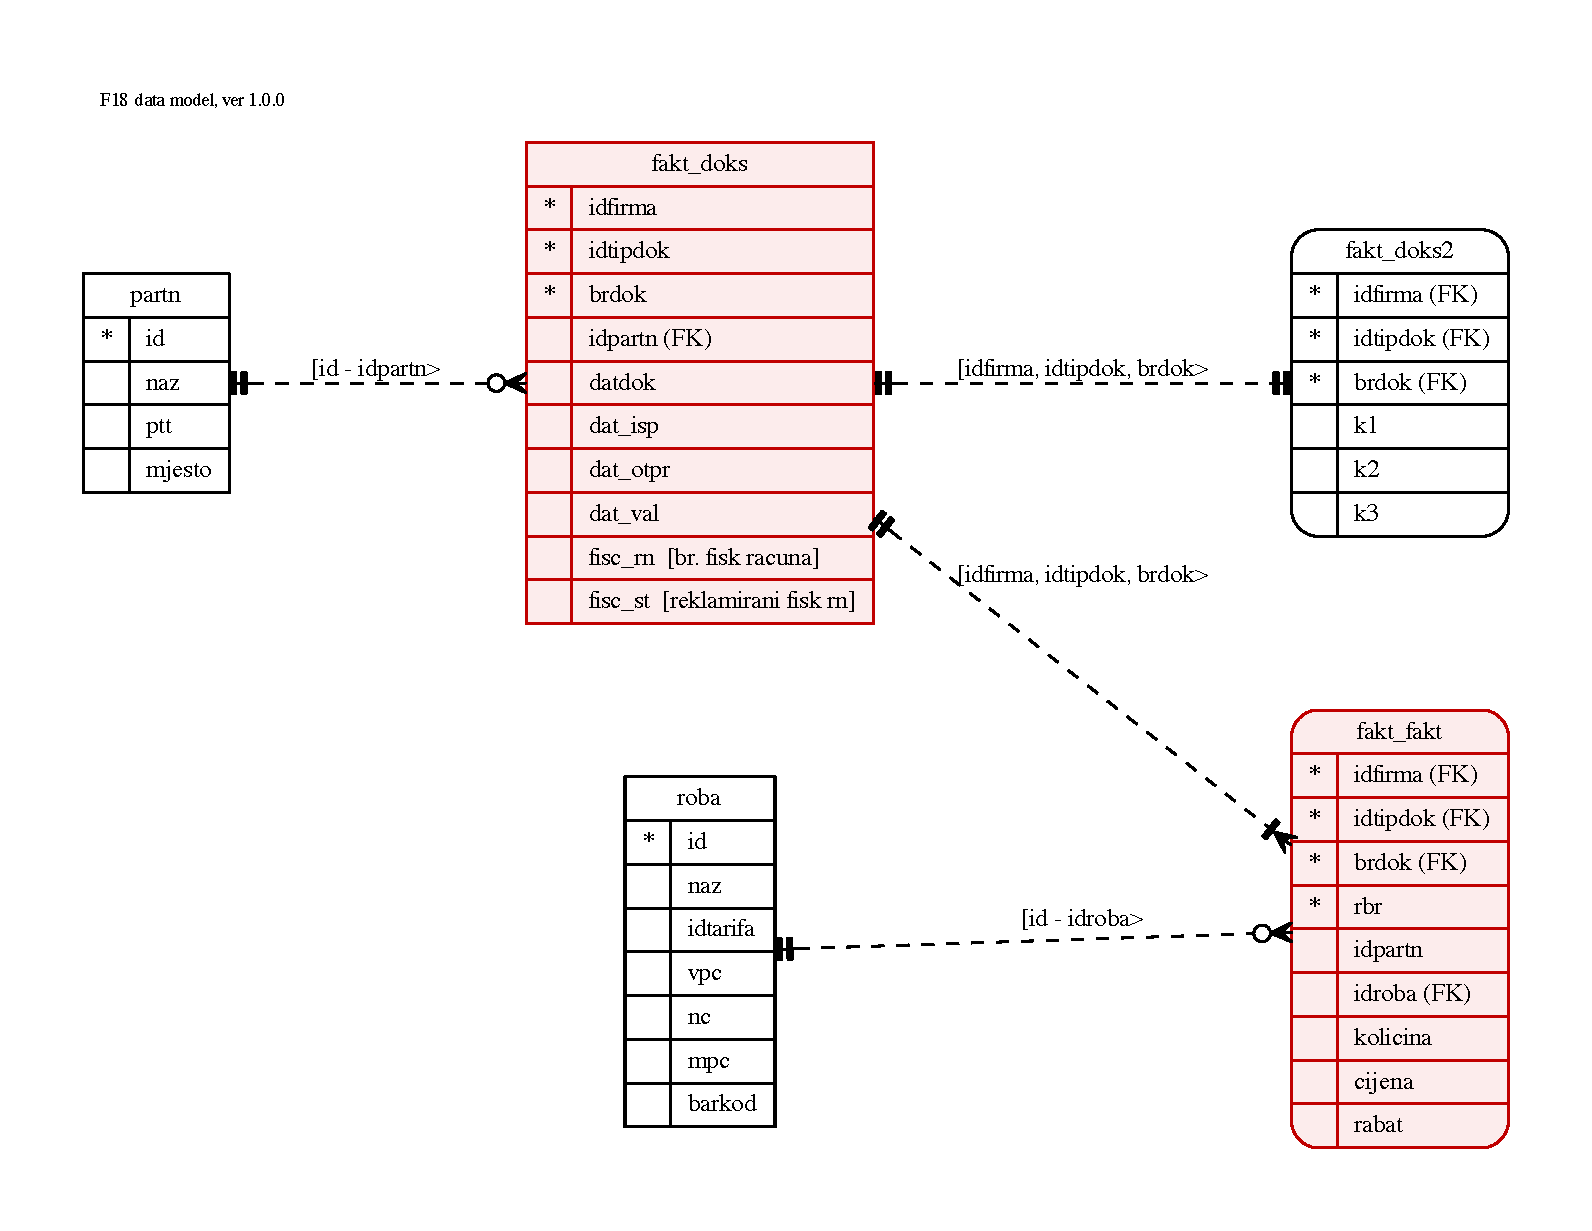
\includegraphics[width=15cm]{img/F18_db.pdf}
\caption{F18 transakcijski db model (relevantni dio)}
\end{figure}


\section{Pentaho}

Pentaho: analysis multidimensional, reporting, dashboards (key performance indicators) \cite[str.~7]{pentaho32}.

\begin{figure}[h]
\centering
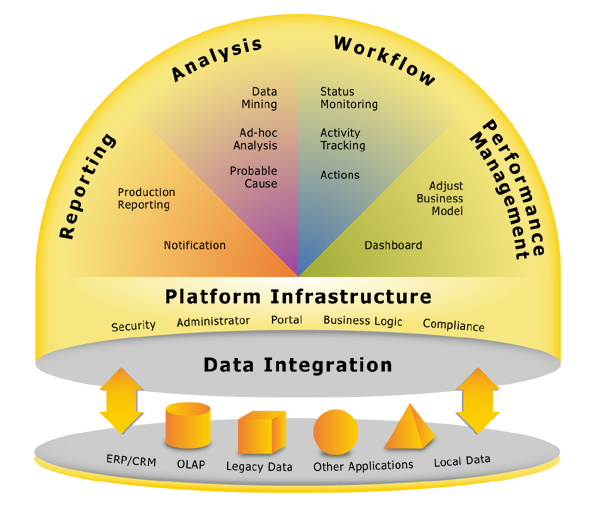
\includegraphics[width=15cm]{img/pentaho_arhitektura_eric.png}
\caption{Pentaho arhitektura (\cite{web:eric})}
\end{figure}



Spoon

data mining weka ?


\subsection{dimension table}

\begin{figure}[h]
\centering
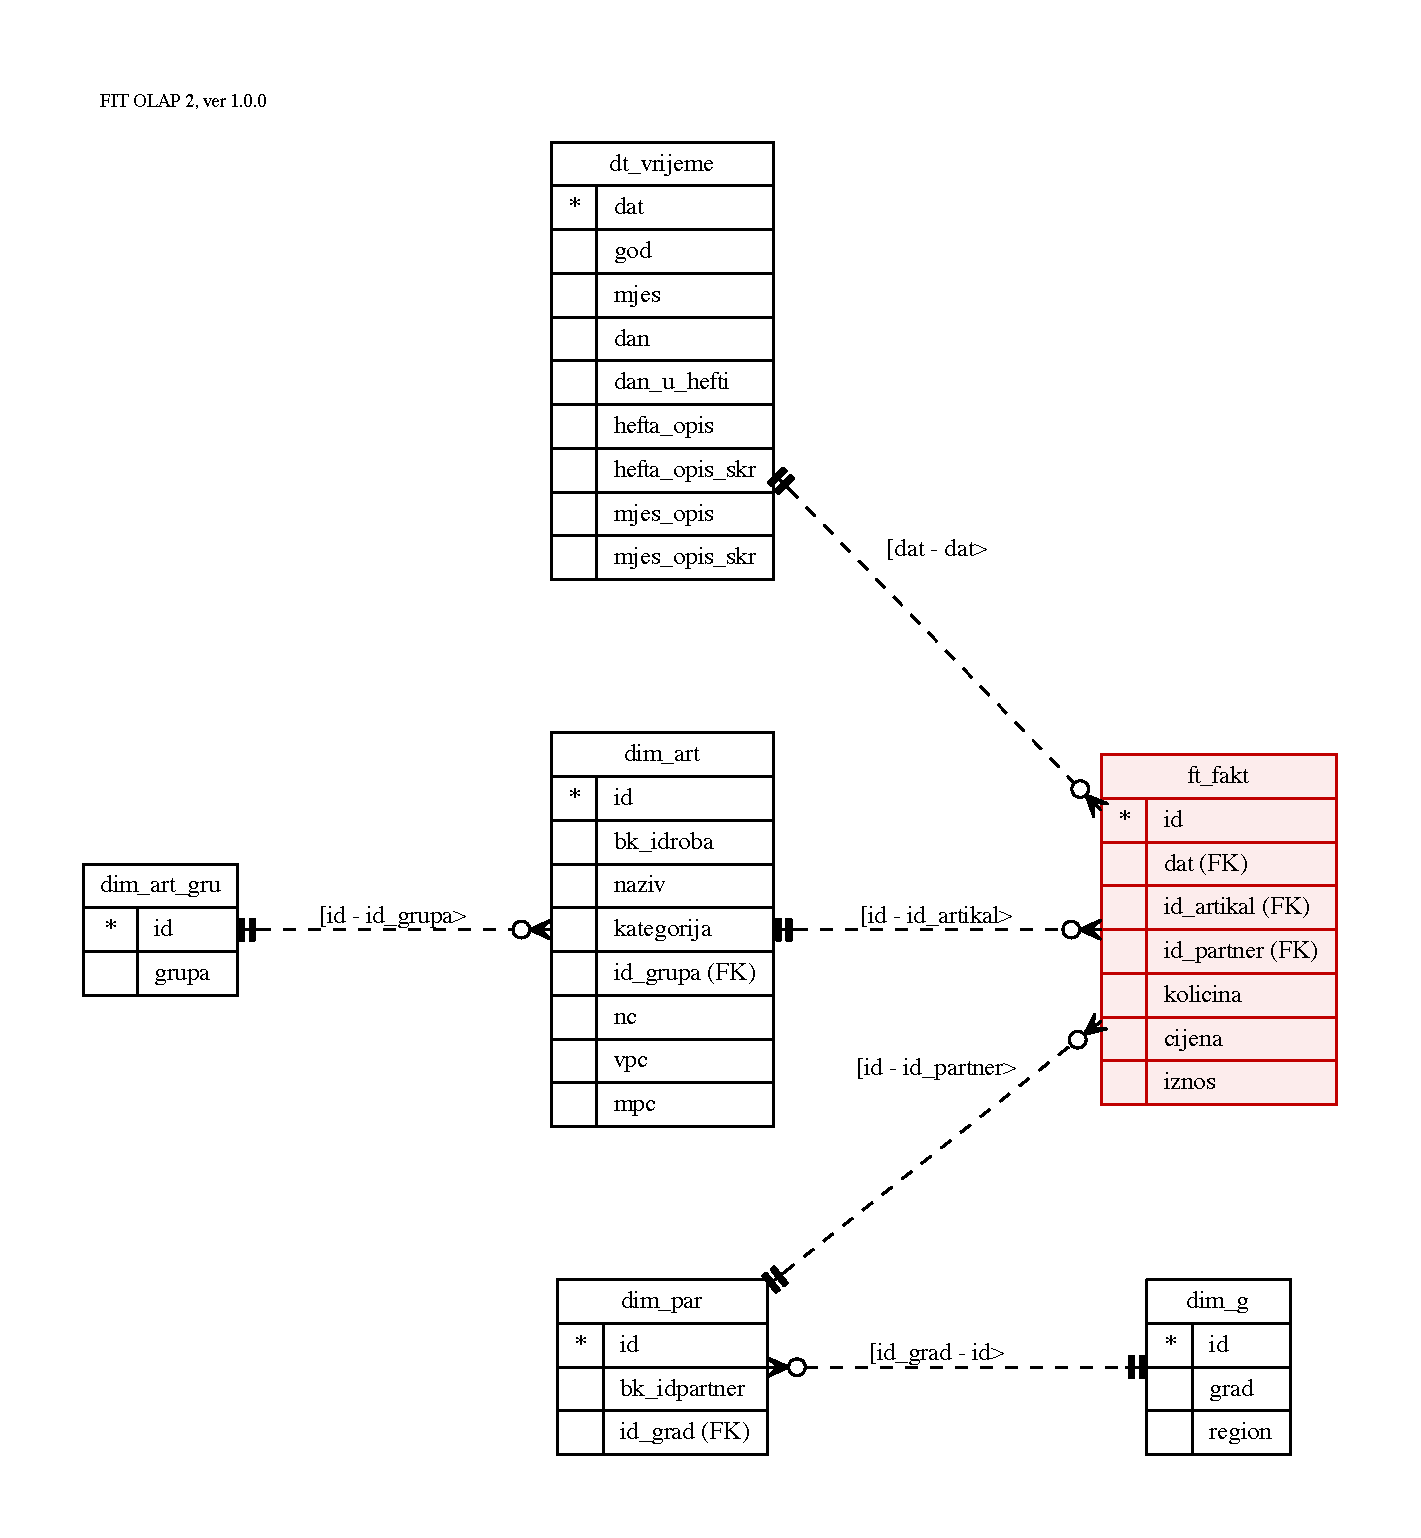
\includegraphics[width=15cm]{img/F18_olap.pdf}
\caption{OLAP schema}
\end{figure}


Mondrian schema:

\begin{figure}[h]
\centering
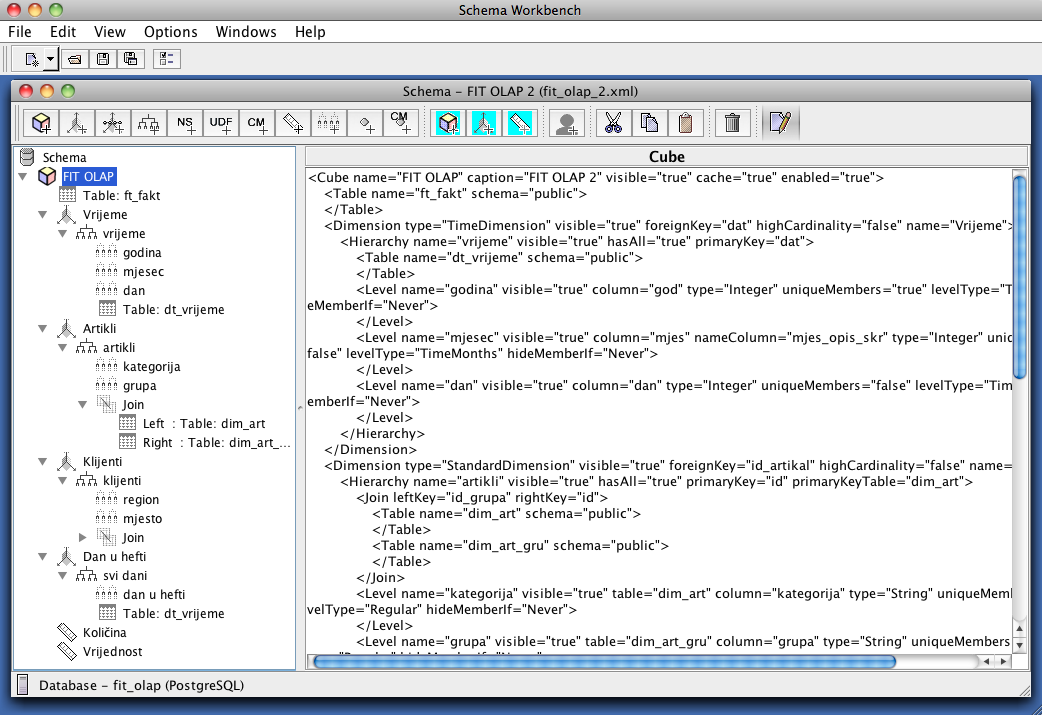
\includegraphics[width=15cm]{img/fit_olap_mondrian_schema}
\caption{Mondrian schema OLAP 2 cube}
\end{figure}




\subsection{facts table}



\subsection{ETL (Extract Transforn Load)}




\section{Poslovna pitanja (Business questions)}

Kolika je prodaja u određenom vremenskom periodu ?

Kakav je odnos prodaje prodaje za određeni period tekuće godine u odnosu na predhodne ?

Koji su efekti zapošljavanja radnika po pitanju ostvarnih prihoda ?


\section{Analiza podataka}

\lstset{ %
   language=SQL,
   basicstyle=\small,
   numbers=left,
   numbersep=5pt,
   breaklines=true,
   backgroundcolor=\color{yellow!15},
   tabsize=2,
   keywordstyle=\color{blue},
   captionpos=b, 
   frame=none
}


\begin{figure}[H]
\centering
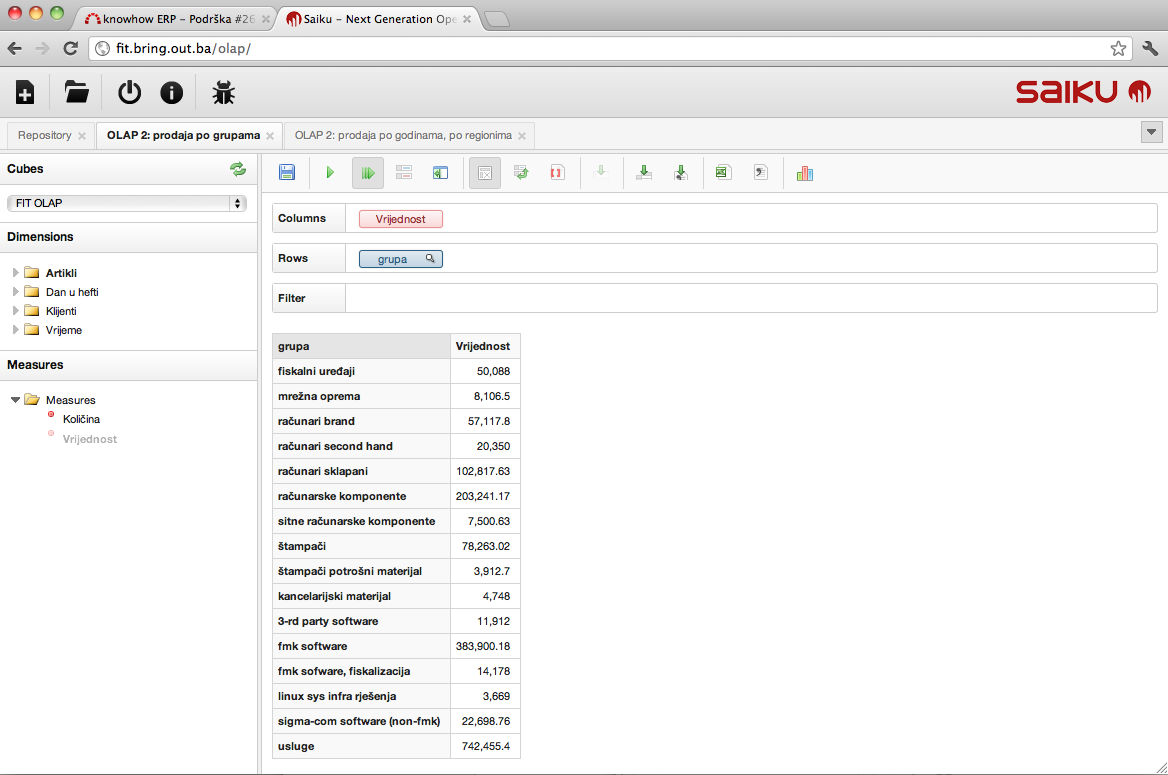
\includegraphics[width=15cm]{img/saiku_rpt_grupe}
\caption{Pregled prodaje po grupama artikala}
\end{figure}

\lstset{caption={Pregled prodaje po grupama artikala}}
\begin{lstlisting}
SELECT
NON EMPTY {Hierarchize({[Measures].[Vrijednost]})} 
ON COLUMNS,
  NON EMPTY {Hierarchize({[Artikli.artikli].[grupa].Members})} 
ON ROWS
FROM [FIT OLAP]
WHERE {Hierarchize({[Vrijeme.vrijeme].[All Vrijeme.vrijemes]})}
\end{lstlisting}


\begin{figure}[H]
\centering
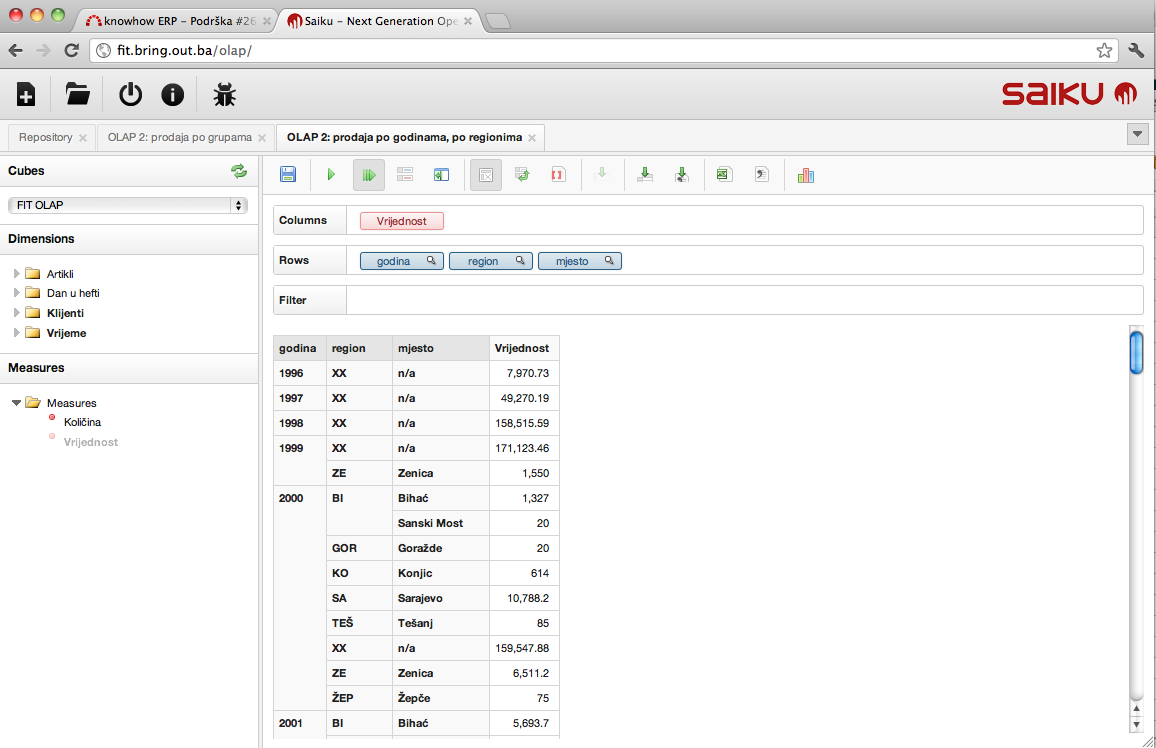
\includegraphics[width=15cm]{img/saiku_rpt_region}
\caption{Pregled prodaje po regionima, po godinama}
\end{figure}

\lstset{caption={Pregled prodaje po regionima}}
\begin{lstlisting}
SELECT
  NON EMPTY {Hierarchize({[Measures].[Vrijednost]})} 
ON COLUMNS,
  NON EMPTY 
    Hierarchize(
      Union(CrossJoin([Vrijeme.vrijeme].[godina].Members, 
      [Klijenti.klijenti].[region].Members), CrossJoin([Vrijeme.vrijeme].[godina].Members, 
      [Klijenti.klijenti].[mjesto].Members))
    ) 
ON ROWS
FROM [FIT OLAP]
\end{lstlisting}



\subsection{Redovi, Kolone, Filteri}





\subsection{Ekspert}

Poznavanje sadržaja i postojećih struktura podataka.





navodim pentaho: \cite{pentaho32}

navodim stranu 215: \cite[str.~215]{pentaho32}

wikipedia olap cube: \cite{web:wikipedia:olap_cube}
wikipedia xmla: \cite{web:wikipedia:xmla}

\chapter{Zaključak}
Zaključak.

\bibliography{literatura}
\bibliographystyle{fit}

\chapter{Rezime}
Rezime.

\appendix

\chapter{Korišteni alati}

\chapter{Pregled toga i toga}

...


\end{document}
